\section{一些功能}

\subsection{快捷键}

\begin{center}
% Table generated by Excel2LaTeX from sheet 'Sheet1'
\begin{table}[htbp!]
  \centering
  \caption{快捷键}
    \begin{tabular}{ll|ll}
    \toprule
    \multicolumn{1}{c}{功能}    & \multicolumn{1}{c}{快捷键}   & \multicolumn{1}{c}{功能}    & \multicolumn{1}{c}{快捷键}\\
    \midrule
    注释          & Ctrl + R              & 切换到Command Window   & Ctrl + 0  \\
    自动排版      & Ctrl + I              & 切换到Command History  & Ctrl + 1 \\
    取消注释      & Ctrl + T              & 切换到 Current Folder  & Ctrl + 2  \\
    向右缩进      & Ctrl + [              & 切换到Workspace        & Ctrl + 3 \\
    向左缩进      & Ctrl + ]              & 切换到Editor           & Ctrl + Shift + 0 \\
    执行当前单元  & Shift + Ctrl + Enter  & Editor之间的切换       & Ctrl + PgDn/PgUp \\
    终止程序      & Ctrl + C              & 添加函数               & Ctrl + J \\
    上一个单元    & Ctrl + Down           & 下一个单元             & Ctrl + Up \\
    \bottomrule
    \end{tabular}%
  % \label{tab:addlabel}%
\end{table}%
\end{center}



\subsection{MATLAB启动}
这里不描述通常的点击图标启动.有这样两种启动方式:
\begindot
  \item \mcode{matlab},完全启动,即正常的启动;
  \item \mcode{matlab -nojvm},只启动Command窗口,这将禁用与java相关的功能,启动速度较快.
\myenddot
在Windows中,可以命令方式来启动,即在cmd或 \mcode{Ctrl+R} 调出的“运行”中执行,对应的命令在其后已经给出.命令启动有个前提, MATLAB的可执行程序路径已经在环境变量中.\par

\begin{figure}[htbp]
  \centering
  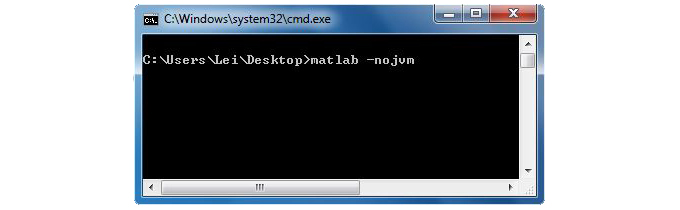
\includegraphics[width=0.9\textwidth]{startmatlab1.jpg}
\end{figure}

\begin{figure}[htbp]
  \centering
  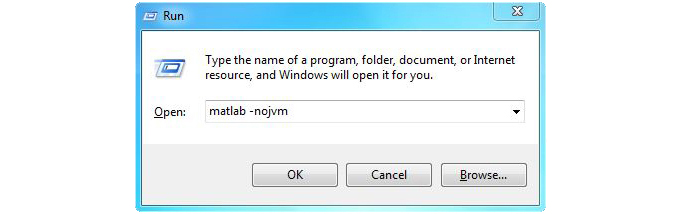
\includegraphics[width=0.9\textwidth]{startmatlab2.jpg}
  \caption{MATLAB “no java” 启动}
\end{figure}

在图中直接输入以 \mcode{matlab} 可实现完全启动.若是期望轻量级编程,可以“no java”方式启动,并配合其他编辑器(比如Sublime Text),可以实现脚本或函数的编辑及执行.对两种方式做个对比:

\begindot
  \item 完全启动,速度慢,功能齐全,占用内存大(相对);
  \item “no java”启动,速度快,功能少一部分,占用内存小.
\myenddot

\notation{MATLAB环境变量的设置.假设MATLAB安装在C:$\backslash$MATLAB目录下,那么, matlab.exe应该在C:$\backslash$MATLAB$\backslash$bin目录下.接着设置环境变量,电脑属性$\rightarrow$高级系统设置$\rightarrow$环境变量$\rightarrow$用户变量下选中PATH并点击编辑按钮$\rightarrow$添加C:$\backslash$MATLAB$\backslash$bin(在最后加入分号添加)$\rightarrow$一路保存退出}.


\subsection{路径设置}
设置路径的方法:
\begindot
  \item 鼠标点击实现. Home$\rightarrow$set path. Add Folder...只添加选定文件夹的路径, Add with Subfolders...添加指定文件夹及其所有子文件夹路径.

    \begin{figure}[htbp]
      \centering
      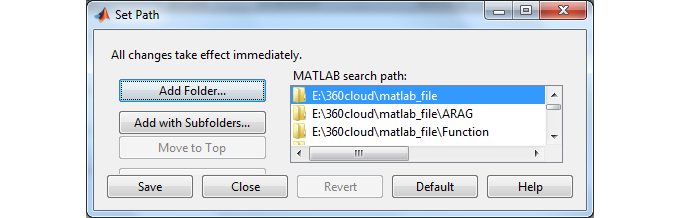
\includegraphics[width=0.9\textwidth]{setpath.png}
      \caption{添加路径}
    \end{figure}

  \item 通过命令添加,比如:

    \vspace{-0.8cm}
    \begin{lstlisting}[caption = 添加路径]
      addpath('D:\matlab_file')
    \end{lstlisting}

\myenddot
添加路径的意义在于,这使得我们期待调用的脚本、函数或资源等能够被找到.

\notation{如果路径中包含空格,用 \mcode{' '} 来表示空格,即两个单引号,中间包含一个空格.}



\subsection{startup}
startup.m是在MATLAB启动时就执行的脚本.若是需要它,我们需要做三件事情:
\begindot
  \item 新建startup.m;
  \item 确保startup.m所在文件夹的路径已经添加;
  \item 编辑需要MATLAB启动就执行的内容.
\myenddot

\vspace{-0.8cm}
\begin{lstlisting}[caption = 我的startup.m]
  clc;                    % 清除Command窗口显示的内容
  cd D:\matlabfile;       % 定位到matlabfile文件夹
  addpath(genpath(pwd));  % 将当前文件夹的所有文件夹及子文件夹添加到路径中
  % pwd为获得当前文件夹路径,即D:$\backslash$matlabfile
\end{lstlisting}
这段代码执行3个命令,主要目的还是在于进入到我的工作目录,并添加可能的新的路径(因而用了 \mcode{genpath}).



\subsection{计时器}
\mcode{tic} 为计时开始, \mcode{toc} 为计时结束.通常用以查看代码/算法执行的时间.

\vspace{-0.8cm}
\begin{lstlisting}[caption = 计时1]
  tic
  disp('Time recorder...');
  toc
\end{lstlisting}

\vspace{-0.8cm}
\begin{lstlisting}[caption=计时2]
  t1 = tic;
  disp('Time recorder...');
  toc(t1)
\end{lstlisting}

\vspace{-0.8cm}
\begin{lstlisting}
  Time recorder...
  Elapsed time is 0.007663 seconds.
\end{lstlisting}

两个例子单独的执行效果如上.在使用时可以注意以下几点:
\begindot
  \item 若是不需要输出时间,在 \mcode{toc} 后加分号即可;
  \item 若需要保存记录的时间,可用变量存储,比如 \mcode{usedtime = toc} 或 \mcode{usedtime = toc(t1)} .
  \item 计时方案2适合有多个计时需求的应用.
\myenddot

\notation{另一种计时 \mcode{etime} ,但这并不是推荐的方式, \mcode{help etime} 查看.}



\subsection{代码单元}
\mcode{\%} 是注释, \mcode{\%\%} 则是一个单元(同时作为注释). 

\vspace{-0.8cm}
\begin{lstlisting}[caption=代码单元]
  %\% display 1
  disp('the first cell.');

  %\% display 2
  disp('the second cell.');
  % 两个百分号与注释之间有空格.
\end{lstlisting}

代码单元可在不选中代码的情况下,可以快捷键 \mcode{Ctrl+Shift+Enter} 连续执行.并还有以下好处:
\begindot
  \item 一个单元一个单元的执行,方便检错/调试;
  \item 方便查看过程数据;
  \item 把具有特定功能的一段代码作为一个单元,使得代码结构清晰.
\myenddot



\subsection{断点调试}
这里是针对function,通过设置断点找出错误所在,亦或了解代码执行过程.在需要暂停的一行或多行前用鼠标点击设置断点.

\begin{figure}[htbp]
  \centering
  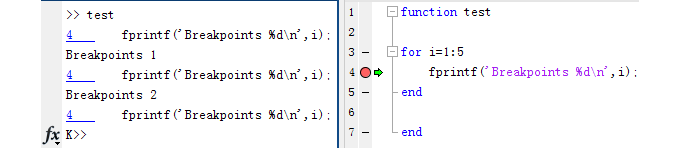
\includegraphics[width=0.9\textwidth]{breakpoint1.png}
\end{figure}

\begin{figure}[htbp]
  \centering
  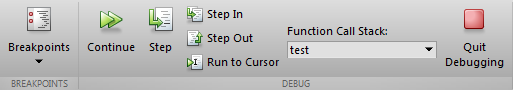
\includegraphics[width=0.9\textwidth]{breakpoint3.png}
  \caption{断点调试}
\end{figure}

相对于通过执行选中代码段来调试,这种方式更加便捷,并且适合批量操作.断点调试常用的两个快捷键:
\begindot
  \item \mcode{F5}, 继续执行;
  \item \mcode{Shift+F5}, 停止继续执行(Quit Debugging).
\myenddot



\subsection{代码发布}
 代码发布,就功能而言,即可用其他文档格式展现代码.发布的格式有多种可选,比如: latex、html、doc、ppt等等.发布方式:
 \begindot
  \item 在菜单栏Publish下设置和发布;
  \item 通过函数 \mcode{publish} 发布,查看 \mcode{help publish}.比如将test.m发布为pdf.

  \vspace{-0.8cm}
  \begin{lstlisting}[caption = 代码发布]
    publish('test.m','pdf');
  \end{lstlisting}

\myenddot

\begin{figure}[htbp]
  \centering
  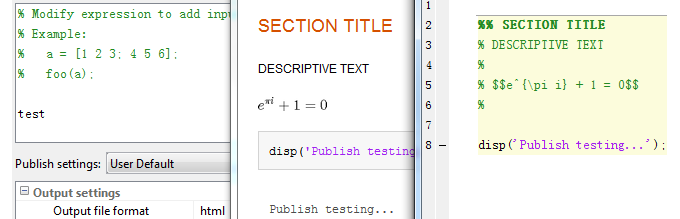
\includegraphics[width=0.9\textwidth]{publish.png}
  \caption{代码发布}
\end{figure}

发布代码的同时,结果也会一同发布,这包括输出和图像等.代码发布还有这样一些细节:
\begindot
  \item 添加章节,使代码更加直观.这可以通过代码单元来实现;
  \item 注释设置,一则可以设置字体,二则可以设置列表(list);
  \item 添加其他元素,比如:图片、公式、超链接.
\myenddot

\notation{就我当前所用版本,要发布含数学公式的建议用\LaTeX,其他几种公式转换为图片发布,效果并不好.或可用其他方式弥补也是可以的(比如先发布为\LaTeX,再生成pdf).也许,这仅仅是因为对\LaTeX的钟爱.}



\subsection{代码保护}
代码保护(protect function)从功能上来理解,有两点:
\begindot
  \item 代码加密(用这种方式生成的文件是被加密的),同时又能像其他文件一样调用;
  \item 预解析文件,直接调用解析过的文件,可以提高执行速度.
\myenddot
首先,通过 \mcode{pcode} 将m文件解析为p后缀文件;然后直接调用该文件.这里给出了针对单个文件的例子,但也可一次解析多个文件.

  \vspace{-0.8cm}
  \begin{lstlisting}[caption = 代码保护]
    pcode filename.m
  \end{lstlisting}

\notation{生成解析文件后,路径下就有两个同名,但是后缀不同的文件.对m文件修改后需要重新解析,不然,会调用较新的m文件,而不是p文件.另外,"解析"一词在这里更多的是指 \mcode{pcode} 的函数作用.}



\subsection{应用发布}
 应用发布是指把脚本或者函数编译成可执行的exe文件.应用发布包含两个步骤:

 \begindot
  \item \mcode{mbuild -setup} 选择和配置编译器;
  \item \mcode{mcc -m myfile.m} 将脚本编译成可执行文件.
 \myenddot

注意上面命令之间的空格.编译得到的同名exe文件在MATLAB安装目录的bin文件夹下,或者在所编译文件所在的文件夹下.

\subsection{警告和错误}
在编写程序时,会用一些输出来标识警告或者错误,以下是针对这个问题的方法.

\vspace{-0.8cm}
\begin{lstlisting}[caption = 红色字符串输出]
  fprintf(2,'edit your text here.');
\end{lstlisting}


\vspace{-0.8cm}
\begin{lstlisting}[caption = 警告输出]
  warning('edit your text here.')};
\end{lstlisting}

\vspace{-0.8cm}
\begin{lstlisting}[caption = 错误输出]
  error('edit your text here.')};
\end{lstlisting}

\notation{\mcode{warning} 和 \mcode{error} 可以像 \mcode{fprintf} 一样输出字符串或者数值.例如: \\
\mcode{str = 'I am a string'; warning('\%s',str)}}